\subsubsection{WPA}

The \gls{wpa} is a security protocol based on a draft of the \gls{ieee} 802.11i amendment. It was pushed by the \gls{wifi} Alliance in 2003 as an intermediate solution to the weaknesses of the \gls{wep} algorithm \cite{wifi_state}, allowing manufacturers to patch existing \gls{wep} devices with a safer authentication mechanism while maintaining interoperability. Since its conception, it was meant to be replaced as soon as the \gls{ieee} 802.11i amendment was published in its definitive form \cite{wpa_whitepaper}.

\gls{wpa} moved away from the 40-bit and 104-bit \gls{wep} keys and adopted two new authentication methods. \gls{wpa}-Personal uses a human-readable passphrase as proof of knowledge to authenticate clients. While \gls{wpa}-Enterprise relies on the \gls{ieee} 802.1X standard to authenticate clients on a remote server using one the \gls{eap} \cite{wpa_whitepaper}. Both authentication mechanisms result in the \gls{pmk}, a key that is used to derive other keys used internally by \gls{wpa} as foundation for its privacy protocols.

\paragraph{PSK}

The \gls{psk} is the authentication protocol of \gls{wpa}-Personal networks \cite{wifi_state}. It derives a 256-bit key \gls{DK} using the \gls{pbkdf2} algorithm \cite{rfc8018} from a sequence \gls{P} of 8 to 63 \gls{ascii}-encoded characters, between ' ' (32) and '$\sim$' (126) \cite{ieee_80211_2020}. On \gls{pbkdf2} invocation, the \gls{ssid} of the network is used as the salt \gls{S}, the iteration count \gls{c} is set to 4096, and the length \gls{dkLen} of \gls{DK} is given in bytes.

\[ \gls{DK} = \gls{pbkdf2}(\gls{P}, \gls{S}, \gls{c}, \gls{dkLen}) \]
\[ \therefore \]
\[ \gls{psk} = \gls{pbkdf2}(\gls{P}, \gls{ssid}, 4096, 256 / 8) \]

\paragraph{TKIP}

The \gls{tkip} is a cipher suite designed to enhance \gls{wep} on existing hardware when \gls{wpa} authentication is configured \cite{ieee_80211_2020}. \gls{tkip} encapsulates the original \gls{wep} algorithm to address all security problems known at the time while complying with the first generation stations' constraint of 4 million instructions per second, about 5 instructions per byte processed.

The \gls{mic} was introduced to detect forgery attacks. It is calculated with the Michael algorithm, that due to the computing constraints, couldn't provide the level of effectiveness desired and was complemented with countermeasures on a latter step of \gls{tkip} \cite{ieee_80211_2020}. The Michael algorithm relies on a key for authentication purposes, either a single 128-bit key is used by both nodes for encryption and decryption or each node has its 64-bit key for encryption, which is shared with the other node for decryption.

The frame order started to be enforced via the \gls{tkip} Sequence Counter to avoid replay attacks. Any \gls{mpdu} received out of sequence is ignored.

\begin{figure}[h]
    \centering
    
\includegraphics[width=\linewidth]{contents/background-in-wireless-networks/protected-network-standards/wpa/tkip/construction-of-expanded-tkip-mpdu.png}
    \caption{Construction of Expanded \gls{tkip} \gls{mpdu}}
    {Source: \cite{ieee_80211_2020}}
    \label{figure:ieee80211_figure43e}
\end{figure}

The original \gls{wep} \gls{mpdu} format was extended, as shown in Figure \ref{figure:ieee80211_figure43e}, to accommodate additional information required by \gls{tkip}, the \gls{eiv} and the \gls{mic}. The \gls{tkip} \gls{eiv} field is placed right after the original \gls{wep} \gls{iv} field and adds an extra 4 octets to the \gls{mpdu}. The \gls{tkip} \gls{mic} increases the \gls{mpdu} size by 8 octets and is located between the original \gls{wep} \gls{pdu} and \gls{wep} \gls{icv} fields.

\begin{figure}[h]
    \centering
    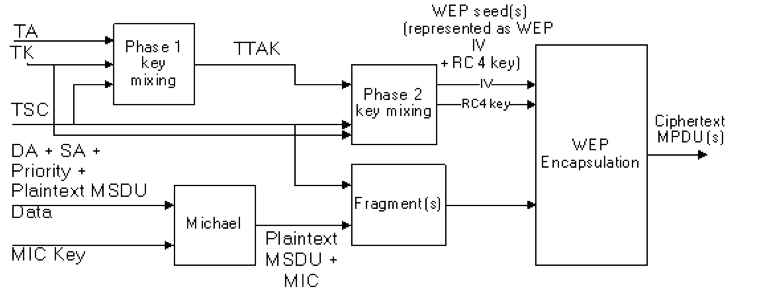
\includegraphics[width=\linewidth]{contents/background-in-wireless-networks/protected-network-standards/wpa/tkip/tkip-encapsulation-block-diagram.png}
    \caption{\gls{tkip} Encapsulation Block Diagram}
    {Source: \cite{ieee_80211_2020}}
    \label{figure:ieee80211_figure43c}
\end{figure}

Represented on Figure \ref{figure:ieee80211_figure43c}, the encryption process of \gls{tkip} combines the \gls{tk}, \gls{ta}, and \gls{tsc} using cryptographic mixing functions and uses it as the \gls{sk} and the \gls{iv} of the \gls{wep} algorithm, effectively enhancing the \gls{prng} seed strength by avoiding the reuse of keys. Then \gls{tkip} calculates the \gls{mic} by executing the Michael algorithm with the \gls{mic} key over the \gls{msdu} plaintext, priority, \gls{sa}, and \gls{da}. The result is fed to the original \gls{wep} algorithm, which outputs the \gls{mpdu} to be transmitted.

\begin{figure}[h]
    \centering
    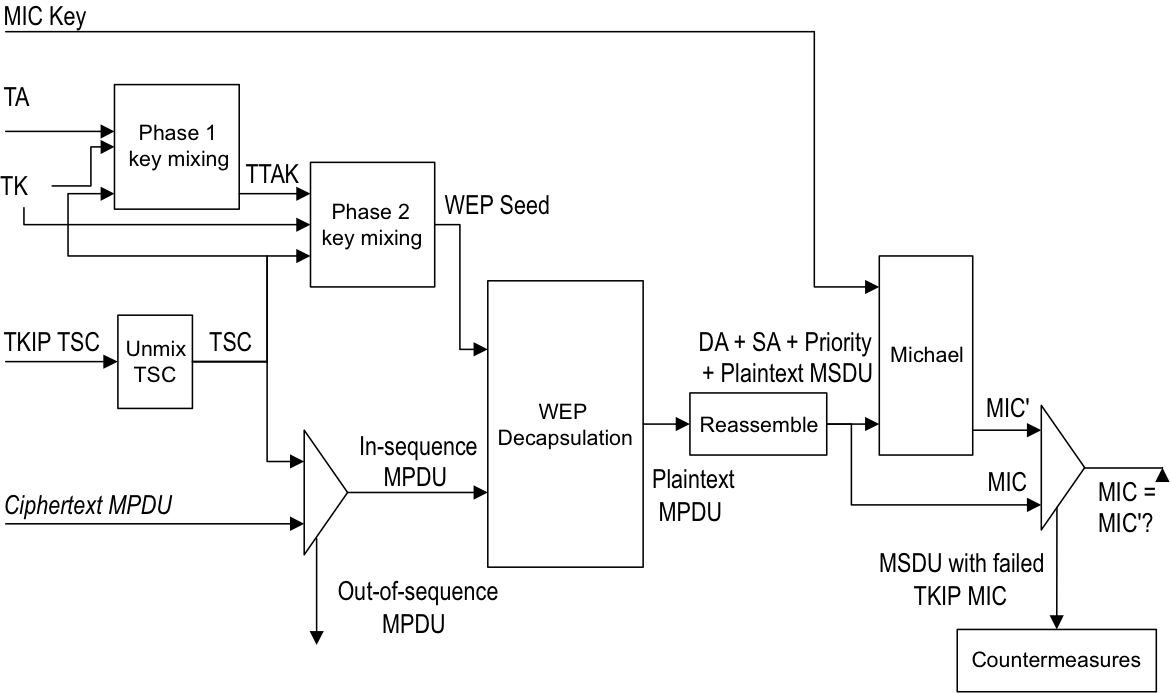
\includegraphics[width=\linewidth]{contents/background-in-wireless-networks/protected-network-standards/wpa/tkip/tkip-decapsulation-block-diagram.png}
    \caption{\gls{tkip} Decapsulation Block Diagram}
    {Source: \cite{ieee_80211_2020}}
    \label{figure:ieee80211_figure43d}
\end{figure}

When decrypting, \gls{tkip} rejects all \glspl{mpdu} received out of sequence. Then it calculates the \gls{wep} seed using the same mixing algorithm of the encryption process. The \gls{wep} algorithm is executed, decrypting the \gls{mpdu}. Michael is executed with the proper \gls{mic} key over the recently recovered data, the result is then compared to the \gls{mic} specified in the \gls{mpdu}. If the \glspl{mic} don't match, \gls{tkip} performs countermeasures procedures to mitigate what looks like an attack. Otherwise, the message is returned by the algorithm, meaning that the \gls{mpdu} was decrypted and successfully authenticated. The decryption mechanism is illustrated on Figure \ref{figure:ieee80211_figure43d}.

\FloatBarrier

\paragraph{Security}

A compromise was made on the \gls{tkip} design to make possible its use on legacy \gls{wep} hardware. The forgery attacks were mitigated with the introduction of the Michael algorithm, but, due to computing power constraints, while blocking the forged packets it would cause a denial of service on the network \cite{ieee_80211_2020}.

As \gls{tkip} just encapsulates the \gls{wep} algorithm, it still relies on the security of the \gls{rc4} \gls{prng}. It was found that the keystream generated by \gls{rc4} is biased towards certain sequences and it made practical attacks against \gls{wpa}-\gls{tkip} networks within an hour \cite{rc4nomore}. The attacker would establish a \gls{tcp} connection with some victim on the network and would repeatedly send identical packets particularly sized with a well-known content over the connection. Then the wireless traffic was captured and filtered to only what would likely be an attacker's packet. Ciphertext statistics were extracted and plaintext likelihoods calculated using a combination of the \gls{fm} and \gls{absab} biases. Finally, the \gls{mic} key is derived from one of the candidates with the correct \gls{icv}, allowing any other packet of the victim to be fully decrypted.

